\subsection{Semantic and Temporal Case Studies}
\label{sec:crosscoder-semantic-temporal}

We next examine DeepSeek feature 4810 and CodeLlama feature 4309, the candidates with the largest correction counts at the highest dose in the preceding experiments. We connect their intervention outcomes to natural activating contexts and to regions associated with the focal failures. This analysis distinguishes a direction that changes generation from an explanation of the behavior it changes; the two case studies provide different levels of explanatory coherence.

\paragraph{Comparison with shuffled directions.}
The preceding comparison uses randomly selected features from the learned CrossCoder dictionary. A complementary question is whether the selected directions outperform coordinate-randomized perturbations rather than other dictionary features. For each target decoder vector, we construct three controls by randomly permuting its coordinates. This preserves its norm and coordinate-value distribution while disrupting its learned orientation. The permutations remain fixed across tasks and doses; absolute cosine similarity to the target and previously accepted controls is constrained to at most 0.05. We apply each control using the same continuous-steering protocol, negative coefficients, task inputs, per-task seeds, generation settings, extraction, and official evaluation as its target. The main comparison uses $\alpha\in\{-1,-2,-3,-4,-5\}$; opposite-sign control results are retained in the replication package.

\begin{figure*}[t]
\centering
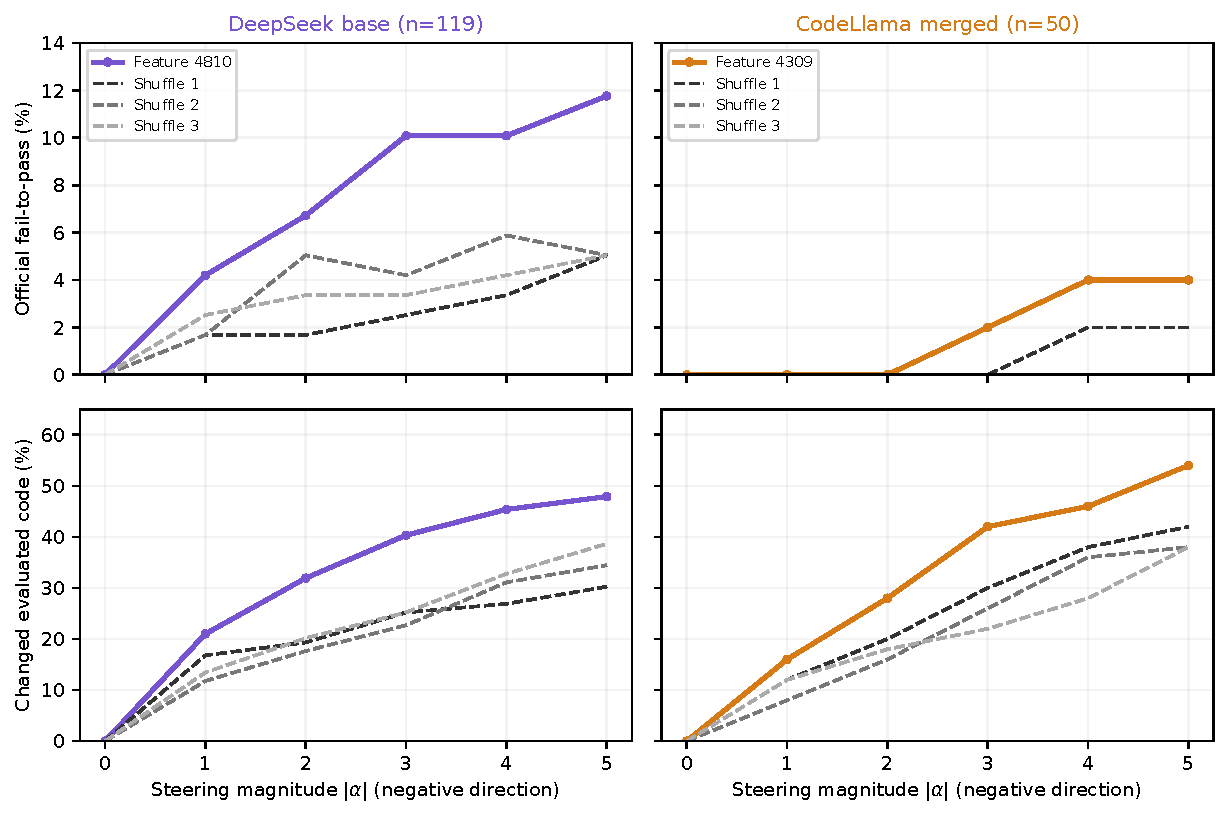
\includegraphics[width=\textwidth]{crosscoder_case_studies/figures/shuffle_corrections_and_changes.pdf}
\caption{Selected directions versus three shuffled-coordinate controls. Columns show DeepSeek feature 4810 and CodeLlama feature 4309; rows show official corrections and changes in extracted, evaluated code. All interventions use the negative direction. The unsteered baseline corrects none of the 119 DeepSeek or 50 CodeLlama tasks. Textual changes can include comments and formatting and do not themselves establish improved correctness.}
\label{fig:case-shuffled-controls}
\end{figure*}

Figure~\ref{fig:case-shuffled-controls} separates correction from output modification. At $\alpha=-5$, DeepSeek feature 4810 corrects 14/119 tasks, compared with 6/119 for each shuffled control, and changes 57 programs, compared with 36, 41, and 46. CodeLlama feature 4309 corrects 2/50 tasks and changes 27 programs; its controls correct 1, 0, and 0 tasks and change 21, 19, and 19 programs. The DeepSeek advantage is therefore clearer than the one-additional-correction advantage in CodeLlama. Corrections under shuffled directions also demonstrate task susceptibility to alternative perturbations. These are descriptive comparisons against three sampled controls under one seed per task, not evidence that the targets outperform every possible random direction.

\paragraph{Natural expression and same-text comparison.}
We first measure how each shared feature is expressed on the original code generated by the two models (Table~\ref{tab:case-natural-expression}). DeepSeek feature 4810 is substantially less expressed on fine-tuned-generated text, whereas CodeLlama feature 4309 has nearly identical mean activation on base- and merged-generated text. These measurements compare different programs encoded in the same latent space; they are not independent model-specific feature activations. Because the cohorts were selected from correctness transitions, this comparison characterizes the selected cases rather than estimating the prevalence of these patterns across arbitrary tasks.

\begin{table}[t]
\centering\small
\caption{Natural expression of the shared feature on different generated texts. Updated denotes fine-tuned for DeepSeek and merged for CodeLlama. Mean activation is averaged over evaluated tokens within each task, then equally over all tasks, including inactive tasks.}
\label{tab:case-natural-expression}
\setlength{\tabcolsep}{4pt}
\begin{tabular}{@{}lrrrr@{}}
\toprule
 & \multicolumn{2}{c}{Tasks with activation} & \multicolumn{2}{c}{Mean activation} \\
\cmidrule(lr){2-3}\cmidrule(l){4-5}
Model / feature & Base text & Updated text & Base text & Updated text \\
\midrule
DeepSeek / 4810 & 119/119 & 75/119 & 0.466 & 0.010 \\
CodeLlama / 4309 & 50/50 & 44/50 & 0.200 & 0.198 \\
\bottomrule
\end{tabular}
\end{table}


To separate text differences from model differences, we also hold each weak-model-generated program fixed and use the residual states obtained when both models replay exactly its token IDs. For feature $j$, we separate the two encoder contributions,
\[
 u_{jt}^{B}=w_{j}^{B\top}h_t^{B},\qquad
 u_{jt}^{V}=w_{j}^{V\top}h_t^{V}.
\]
Their sum, plus the shared encoder bias, enters the joint ReLU and TopK bottleneck. The individual terms are not separately gated sparse activations, and a negative contribution is not a negative sparse activation. Table~\ref{tab:case-same-text} averages these terms within $\pm10$ tokens of the behavioral anchor defined below, first within each task and then across tasks.

\begin{table}[t]
\centering\small
\caption{Same-text encoder contributions within $\pm10$ tokens of the selected anchor. Both models replay the identical weak-model text: base-generated for DeepSeek, merged-generated for CodeLlama. These are terms of one joint encoder preactivation, not independent sparse activations.}
\label{tab:case-same-text}
\setlength{\tabcolsep}{4pt}
\begin{tabular}{@{}lrrr@{}}
\toprule
 & \multicolumn{2}{c}{Mean encoder contribution} & \\
\cmidrule(lr){2-3}
Model / feature & Base model & Updated model & Updated lower \\
\midrule
DeepSeek / 4810 & 0.928 & 0.631 & 103/119 \\
CodeLlama / 4309 & -1.125 & -0.504 & 4/48 \\
\bottomrule
\end{tabular}
\end{table}


Under the same original base text, the fine-tuned DeepSeek model contributes less near the marker in 103/119 cases. Under the same original merged text, CodeLlama merged contributes more, or less negatively, than base in 44/48 aligned cases. These localized readouts complement the natural-text measurements but are not interchangeable with them. Additional normalized and fixed-direction projections are reported in the package; for CodeLlama, decoder-alignment conclusions depend on the readout direction. We therefore do not interpret the table as a universal increase or decrease in an independently measured feature activation.

\paragraph{Locating the behavioral boundary.}
For DeepSeek, we define a reproducible lexical anchor as the first visible token of the earliest line matching a generated test-file comment (\texttt{\#tests/...}, \texttt{\#test/...}, or \texttt{\#test\_task...}), an import of the form \texttt{from task\_func import}, or a \texttt{class Test...(...)} declaration. Leading blank lines and indentation are excluded from the anchor. Comments alone match 107/119 original texts; adding the import condition reaches 117/119, and the class condition recovers the remaining two. This is a marker of a test-like continuation, not a correctness rule: a comment is harmless by itself, and a valid solution can contain later imports or helper definitions.

For CodeLlama, no comparably uniform lexical precursor captures the heterogeneous failures. We instead reuse case-specific regions identified from generated code and evaluation evidence: 16 traceback-confirmed execution-site cases, 18 provisionally identified lines or intervals, and 16 omission regions. These are not validated earliest semantic errors; an omission need not have a unique offending token. Exact character-block alignment transfers region starts from the re-extracted baseline to the frozen activation source. Two starts cannot be aligned safely, so the local same-text comparison uses 48 cases and retains all 50 in whole-text analyses.

\begin{figure*}[t]
\centering
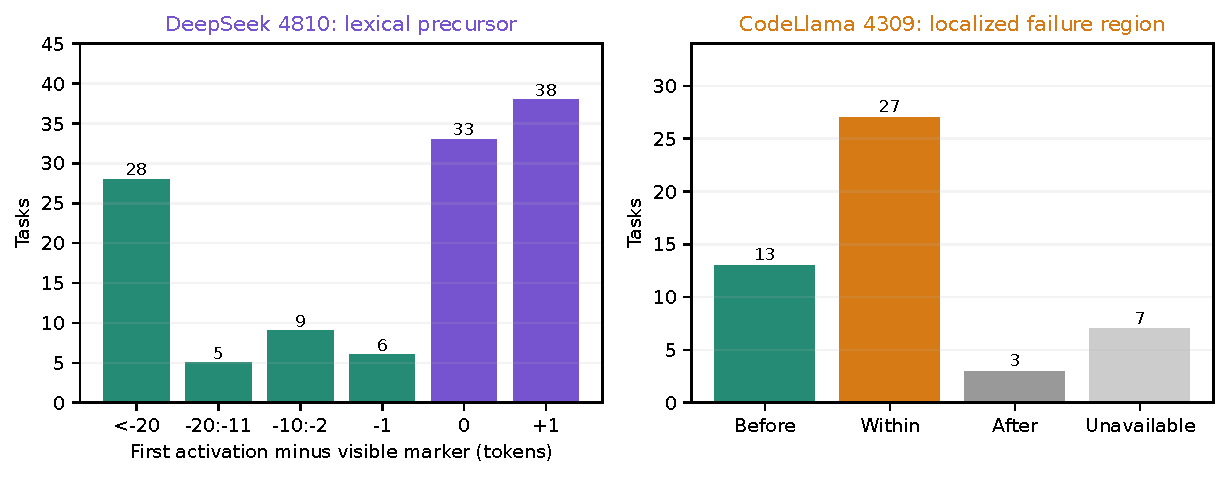
\includegraphics[width=\textwidth]{crosscoder_case_studies/figures/temporal_relation_to_behavior.pdf}
\caption{Natural first activation relative to the focal behavior. Left: signed token distance from the visible DeepSeek test/import marker; negative values precede the marker. The leftmost bins retain earlier activations rather than discarding them. Right: first mapped CodeLlama activation before, within, or after its localized failure region; unavailable combines six inactive texts and one unaligned activation. The two anchors have different evidential status and must not be interpreted as equivalent semantic-error onsets.}
\label{fig:case-temporal-boundaries}
\end{figure*}

DeepSeek first activation lies within one token of the visible marker in 77/119 tasks (Figure~\ref{fig:case-temporal-boundaries}). Of the 107 texts whose first marker is a matching comment, activation begins before the comment in 36 and within its text in 71; none begins after that line. This distinction matters: activation inside a comment can still precede the later import that causes a failure. In all 14 tasks corrected at $\alpha=-5$, the baseline evaluator reports a missing module (\texttt{task\_func} or \texttt{task}), and the original first activation precedes the earliest textual import of that module by 4--29 tokens. This is temporal evidence relative to a failure-associated operation, not proof that the natural feature mediates the failure.

CodeLlama exhibits a different relationship: 13 activations precede the localized region, 27 occur within it, three follow it, and seven are unavailable. In both corrected tasks, /183 and /490, the first captured activation is the newline after an already-written return expression. Continuous steering acts at earlier positions too; its ability to rewrite that expression therefore does not establish that the observed later activation originally caused the incomplete implementation.

\paragraph{Tokens and semantic interpretation.}
Figure~\ref{fig:case-token-contexts} relates these positions to actual token contexts. DeepSeek activation mass includes tokens such as \texttt{import}, \texttt{from}, \texttt{test}, filename fragments, and newlines. The cloud displays activating-token evidence, not a frequency-controlled correlation or a unique semantic definition. In the passing fine-tuned texts, remaining activations also occur around valid example-usage comments and imports, as well as occasional tokens inside the implementation. A more appropriate hypothesis is a direction associated with test-like or illustrative continuation after a solution, rather than a feature that exclusively represents incorrect imports.

\begin{figure*}[t]
\centering
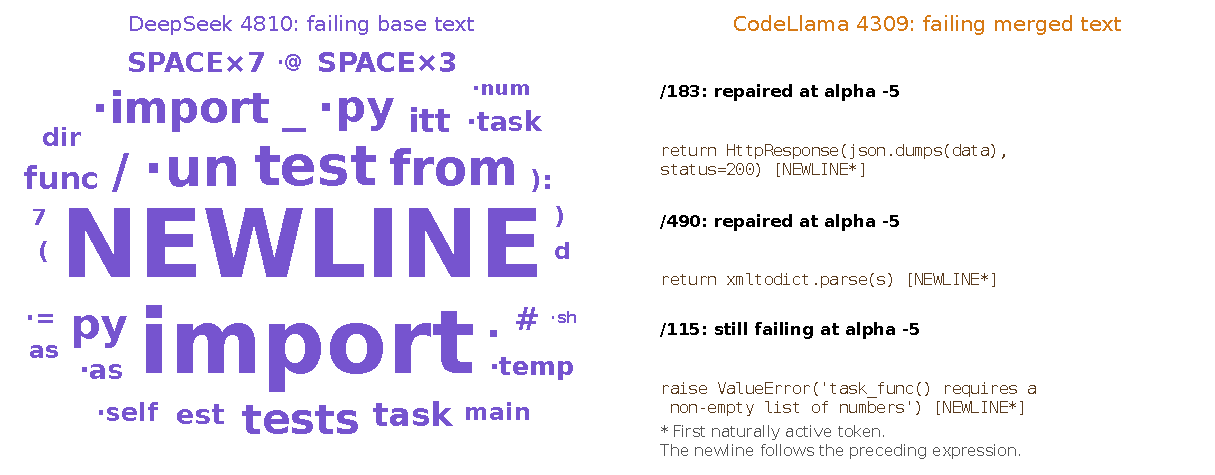
\includegraphics[width=\textwidth]{crosscoder_case_studies/figures/token_cloud_and_return_contexts.pdf}
\caption{Complementary token evidence. Left: DeepSeek 4810 cloud on the 119 original failing base texts; font size increases with the square root of summed activation mass, and tokens require support in at least three tasks. \texttt{NEWLINE} is a visible token alias and a middle dot denotes a space. Right: CodeLlama 4309 first-active newline contexts from failing merged text, including two subsequently corrected tasks and a still-failing counterexample. The snippets describe natural activation, not an activation-gated intervention.}
\label{fig:case-token-contexts}
\end{figure*}

CodeLlama activation is dominated by newline contexts. Among the captured merged-text tokens, 49/51 newlines ending a main-function return statement activate 4309, compared with 92/327 other newline-containing tokens. However, 48/53 return-ending newlines also activate it in the passing base texts. The association is therefore compatible with a structural boundary, not an error detector. The \texttt{raise} example in Figure~\ref{fig:case-token-contexts} further illustrates that activation is not exclusive to returns.

\paragraph{What steering changes.}
The code changes provide a final check on these interpretations (Figure~\ref{fig:case-code-changes}). At $\alpha=-5$, all 14 corrected DeepSeek programs lose the specific markers detected by the heuristic. Eleven originally contained a matching test-file comment, and all eleven lose it. Eight preserve the first main-function body's AST, ignoring comments and the docstring; six also change that body, so their correction cannot be attributed solely to removing trailing code. Marker removal is not sufficient for success: 23 programs lose all heuristic markers but nine remain incorrect.

\begin{figure*}[t]
\centering
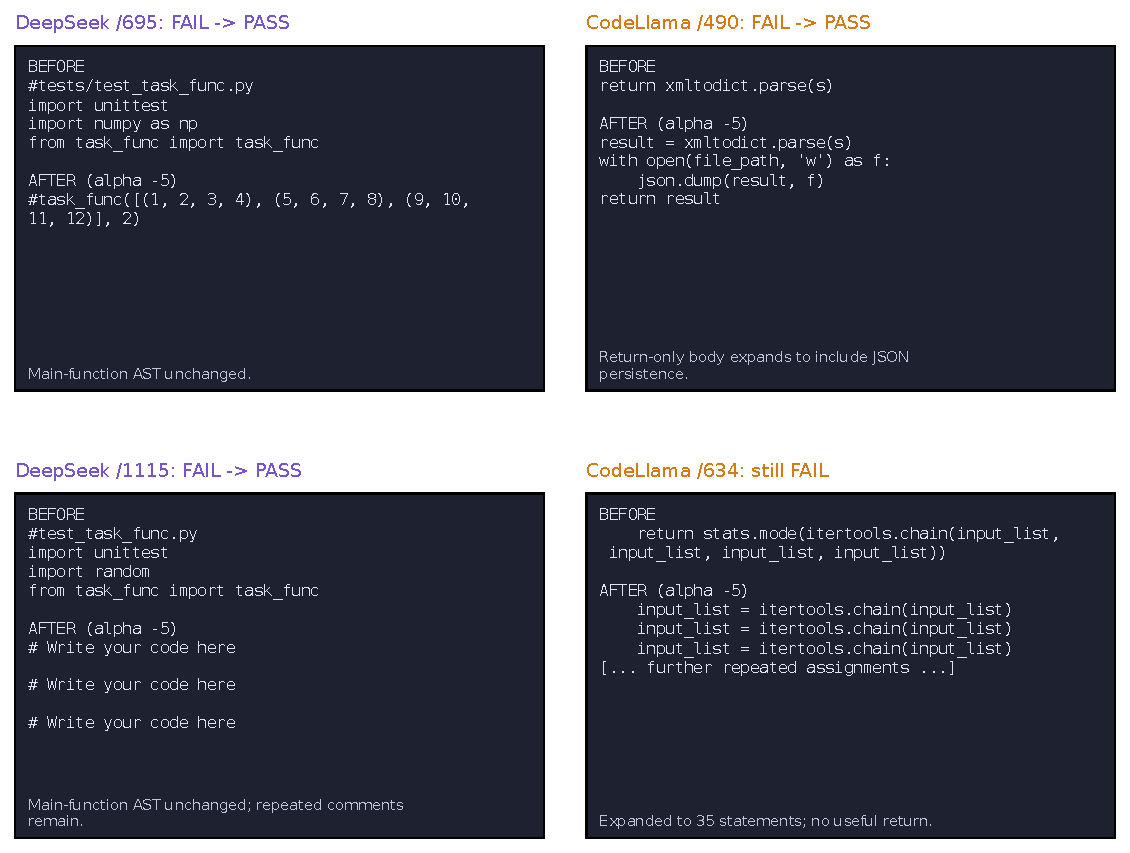
\includegraphics[width=\textwidth]{crosscoder_case_studies/figures/paired_code_examples.pdf}
\caption{Evaluated-code excerpts before and after $\alpha=-5$ steering. DeepSeek /695 removes the test/import continuation while preserving the main-function AST; /1115 replaces it with repeated comments and passes despite continued generation. CodeLlama /490 expands a return-only implementation to restore required JSON persistence, whereas /634 expands into repetition and still fails. Displayed bracketed omissions are editorial; complete programs and diffs are provided in the replication package.}
\label{fig:case-code-changes}
\end{figure*}

DeepSeek /695 replaces tests and an invalid module import with a commented example. In /1115, repeated \texttt{\# Write your code here} comments remain, but the failing test/import block disappears. In /666, executable examples remain and the program passes. These cases support redirection away from the harmful continuation, not a claim that steering necessarily makes the model stop or produces globally cleaner code.

For CodeLlama, /183 replaces a short return with response construction, a required UUID header, and a return, while avoiding double serialization. In /490, steering adds JSON-file persistence before returning the parsed XML. Neither task is corrected by the six shuffled arms at magnitude five. Yet the same structural hypothesis has counterexamples: /634 expands into repetitive assignments without a useful return; /371 and /738 retain their original return-only bodies; and /931 loses its return. Thus, implementation expansion is neither a universal effect nor a sufficient explanation of correctness.

Taken together, the DeepSeek evidence is consistent with a learned direction associated with post-solution test-like continuation: natural token contexts and timing locate it near that transition, same-text readouts distinguish the models there, and steering can redirect the continuation before a failing import appears. For CodeLlama, the evidence supports more limited, task-specific causal leverage over implementation structure. It does not establish a general incomplete-implementation feature or a single mechanism for the regression cohort. The detailed analyses, control arms, code excerpts, and readout sensitivities are available in our replication package~\cite{CrossCoderReplication}.

\subsection{Summary of Evidence}
\label{sec:crosscoder-evidence-summary}

The study provides a path from ReCatcher's behavioral contrasts to testable internal directions. Error-focused screening reduces the latent search space; natural activations, tokens, and temporal anchors motivate semantic hypotheses; and controlled decoder-direction interventions test whether those hypotheses offer practical leverage over code generation and official correctness. Table~\ref{tab:case-evidence-summary} separates these forms of evidence rather than treating them as interchangeable.

\begin{table*}[t]
\centering\small
\caption{Evidence obtained in the two focused case studies. Results are conditional on the selected cohorts and tested directions; they are not a causal decomposition of every model-update effect.}
\label{tab:case-evidence-summary}
\setlength{\tabcolsep}{4pt}
\begin{tabular}{@{}p{0.16\textwidth}p{0.38\textwidth}p{0.38\textwidth}@{}}
\toprule
Evidence & DeepSeek / 4810 & CodeLlama / 4309 \\
\midrule
Natural expression & Much lower shared activation on fine-tuned-generated texts. & Similar mean shared activation on base- and merged-generated texts. \\
Temporal and semantic context & Activation near a test-like continuation and before imports associated with observed failures. & Preference for return-line newlines in both passing and failing texts; activation follows the return in both corrected cases. \\
Controlled intervention & 14/119 corrections at $\alpha=-5$, versus 6/119 per shuffled control. & 2/50 corrections, versus 1/50 for the strongest shuffled control; two distinct task-specific repairs. \\
Interpretive scope & Coherent evidence for redirecting a particular harmful continuation, without proving natural mediation. & Causal leverage on selected implementations, without a general explanation of heterogeneous regressions. \\
\bottomrule
\end{tabular}
\end{table*}

The strongest conclusion is that selected internal directions can be linked to interpretable code-generation patterns and can causally change benchmark outcomes. DeepSeek provides the clearer convergence of behavioral association, natural representation, temporal context, and useful intervention. CodeLlama demonstrates why these links must be tested separately: a direction can repair specific programs without serving as a general detector or explanation of the surrounding failure population.

Random learned features and shuffled-coordinate controls address different alternatives: the former test the usefulness of candidate selection within the latent dictionary, whereas the latter test the learned orientation against matched coordinate-randomized perturbations. Neither comparison, particularly with three controls and one seed per task, proves that the selected direction is uniquely responsible for the model difference. Selection and follow-up also reuse the same cohorts. The results therefore support a reusable, auditable methodology for investigating and manipulating selected behavioral differences, while broader claims require additional tasks, seeds, and experiments isolating natural causal mediation.
